% Options for packages loaded elsewhere
\PassOptionsToPackage{unicode}{hyperref}
\PassOptionsToPackage{hyphens}{url}
\PassOptionsToPackage{dvipsnames,svgnames,x11names}{xcolor}
%
\documentclass[
]{article}
\usepackage{amsmath,amssymb}
\usepackage{iftex}
\ifPDFTeX
  \usepackage[T1]{fontenc}
  \usepackage[utf8]{inputenc}
  \usepackage{textcomp} % provide euro and other symbols
\else % if luatex or xetex
  \usepackage{unicode-math} % this also loads fontspec
  \defaultfontfeatures{Scale=MatchLowercase}
  \defaultfontfeatures[\rmfamily]{Ligatures=TeX,Scale=1}
\fi
\usepackage{lmodern}
\ifPDFTeX\else
  % xetex/luatex font selection
\fi
% Use upquote if available, for straight quotes in verbatim environments
\IfFileExists{upquote.sty}{\usepackage{upquote}}{}
\IfFileExists{microtype.sty}{% use microtype if available
  \usepackage[]{microtype}
  \UseMicrotypeSet[protrusion]{basicmath} % disable protrusion for tt fonts
}{}
\makeatletter
\@ifundefined{KOMAClassName}{% if non-KOMA class
  \IfFileExists{parskip.sty}{%
    \usepackage{parskip}
  }{% else
    \setlength{\parindent}{0pt}
    \setlength{\parskip}{6pt plus 2pt minus 1pt}}
}{% if KOMA class
  \KOMAoptions{parskip=half}}
\makeatother
\usepackage{xcolor}
\usepackage[margin=1in]{geometry}
\usepackage{color}
\usepackage{fancyvrb}
\newcommand{\VerbBar}{|}
\newcommand{\VERB}{\Verb[commandchars=\\\{\}]}
\DefineVerbatimEnvironment{Highlighting}{Verbatim}{commandchars=\\\{\}}
% Add ',fontsize=\small' for more characters per line
\usepackage{framed}
\definecolor{shadecolor}{RGB}{248,248,248}
\newenvironment{Shaded}{\begin{snugshade}}{\end{snugshade}}
\newcommand{\AlertTok}[1]{\textcolor[rgb]{0.94,0.16,0.16}{#1}}
\newcommand{\AnnotationTok}[1]{\textcolor[rgb]{0.56,0.35,0.01}{\textbf{\textit{#1}}}}
\newcommand{\AttributeTok}[1]{\textcolor[rgb]{0.13,0.29,0.53}{#1}}
\newcommand{\BaseNTok}[1]{\textcolor[rgb]{0.00,0.00,0.81}{#1}}
\newcommand{\BuiltInTok}[1]{#1}
\newcommand{\CharTok}[1]{\textcolor[rgb]{0.31,0.60,0.02}{#1}}
\newcommand{\CommentTok}[1]{\textcolor[rgb]{0.56,0.35,0.01}{\textit{#1}}}
\newcommand{\CommentVarTok}[1]{\textcolor[rgb]{0.56,0.35,0.01}{\textbf{\textit{#1}}}}
\newcommand{\ConstantTok}[1]{\textcolor[rgb]{0.56,0.35,0.01}{#1}}
\newcommand{\ControlFlowTok}[1]{\textcolor[rgb]{0.13,0.29,0.53}{\textbf{#1}}}
\newcommand{\DataTypeTok}[1]{\textcolor[rgb]{0.13,0.29,0.53}{#1}}
\newcommand{\DecValTok}[1]{\textcolor[rgb]{0.00,0.00,0.81}{#1}}
\newcommand{\DocumentationTok}[1]{\textcolor[rgb]{0.56,0.35,0.01}{\textbf{\textit{#1}}}}
\newcommand{\ErrorTok}[1]{\textcolor[rgb]{0.64,0.00,0.00}{\textbf{#1}}}
\newcommand{\ExtensionTok}[1]{#1}
\newcommand{\FloatTok}[1]{\textcolor[rgb]{0.00,0.00,0.81}{#1}}
\newcommand{\FunctionTok}[1]{\textcolor[rgb]{0.13,0.29,0.53}{\textbf{#1}}}
\newcommand{\ImportTok}[1]{#1}
\newcommand{\InformationTok}[1]{\textcolor[rgb]{0.56,0.35,0.01}{\textbf{\textit{#1}}}}
\newcommand{\KeywordTok}[1]{\textcolor[rgb]{0.13,0.29,0.53}{\textbf{#1}}}
\newcommand{\NormalTok}[1]{#1}
\newcommand{\OperatorTok}[1]{\textcolor[rgb]{0.81,0.36,0.00}{\textbf{#1}}}
\newcommand{\OtherTok}[1]{\textcolor[rgb]{0.56,0.35,0.01}{#1}}
\newcommand{\PreprocessorTok}[1]{\textcolor[rgb]{0.56,0.35,0.01}{\textit{#1}}}
\newcommand{\RegionMarkerTok}[1]{#1}
\newcommand{\SpecialCharTok}[1]{\textcolor[rgb]{0.81,0.36,0.00}{\textbf{#1}}}
\newcommand{\SpecialStringTok}[1]{\textcolor[rgb]{0.31,0.60,0.02}{#1}}
\newcommand{\StringTok}[1]{\textcolor[rgb]{0.31,0.60,0.02}{#1}}
\newcommand{\VariableTok}[1]{\textcolor[rgb]{0.00,0.00,0.00}{#1}}
\newcommand{\VerbatimStringTok}[1]{\textcolor[rgb]{0.31,0.60,0.02}{#1}}
\newcommand{\WarningTok}[1]{\textcolor[rgb]{0.56,0.35,0.01}{\textbf{\textit{#1}}}}
\usepackage{graphicx}
\makeatletter
\def\maxwidth{\ifdim\Gin@nat@width>\linewidth\linewidth\else\Gin@nat@width\fi}
\def\maxheight{\ifdim\Gin@nat@height>\textheight\textheight\else\Gin@nat@height\fi}
\makeatother
% Scale images if necessary, so that they will not overflow the page
% margins by default, and it is still possible to overwrite the defaults
% using explicit options in \includegraphics[width, height, ...]{}
\setkeys{Gin}{width=\maxwidth,height=\maxheight,keepaspectratio}
% Set default figure placement to htbp
\makeatletter
\def\fps@figure{htbp}
\makeatother
\setlength{\emergencystretch}{3em} % prevent overfull lines
\providecommand{\tightlist}{%
  \setlength{\itemsep}{0pt}\setlength{\parskip}{0pt}}
\setcounter{secnumdepth}{-\maxdimen} % remove section numbering
\ifLuaTeX
  \usepackage{selnolig}  % disable illegal ligatures
\fi
\IfFileExists{bookmark.sty}{\usepackage{bookmark}}{\usepackage{hyperref}}
\IfFileExists{xurl.sty}{\usepackage{xurl}}{} % add URL line breaks if available
\urlstyle{same}
\hypersetup{
  pdftitle={STAT 847: Analysis Assignment 2},
  colorlinks=true,
  linkcolor={Maroon},
  filecolor={Maroon},
  citecolor={Blue},
  urlcolor={blue},
  pdfcreator={LaTeX via pandoc}}

\title{STAT 847: Analysis Assignment 2}
\usepackage{etoolbox}
\makeatletter
\providecommand{\subtitle}[1]{% add subtitle to \maketitle
  \apptocmd{\@title}{\par {\large #1 \par}}{}{}
}
\makeatother
\subtitle{Chris Binoi Verghese ID: 21092999}
\author{}
\date{\vspace{-2.5em}}

\begin{document}
\maketitle

\begin{Shaded}
\begin{Highlighting}[]
\FunctionTok{library}\NormalTok{(randomForest)}
\FunctionTok{library}\NormalTok{(rpart)}
\FunctionTok{library}\NormalTok{(rpart.plot)}
\FunctionTok{library}\NormalTok{(leaps)}
\FunctionTok{library}\NormalTok{(factoextra)}
\FunctionTok{library}\NormalTok{(car)}
\end{Highlighting}
\end{Shaded}

\begin{enumerate}
\def\labelenumi{\arabic{enumi}.}
\tightlist
\item
  (4 points) Using the \texttt{randomForest} function in
  \texttt{library(randomForest)}, make five random forests, each one
  using one of the phenotype variable \texttt{Perimeter\_Growth} as a
  response y variable. The forest should use all 10,000 of the gene
  variables (These are the 9th, \ldots{} , 10,008th variables). Give
  your forest 500 trees, have each tree use 300 gene variables, and set
  a minimum node size of 1. Sample with replacement. Report the
  percentage of variance explained by the forest using \texttt{print()}.
\end{enumerate}

\begin{Shaded}
\begin{Highlighting}[]
\NormalTok{dat }\OtherTok{=} \FunctionTok{read.csv}\NormalTok{(}\StringTok{"F1{-}Hybrids\_Pheno\_10000genes.csv"}\NormalTok{)}
\NormalTok{genes }\OtherTok{=}\NormalTok{ dat[,}\DecValTok{9}\SpecialCharTok{:}\DecValTok{10008}\NormalTok{]}
\NormalTok{pheno }\OtherTok{=}\NormalTok{ dat[,}\DecValTok{1}\SpecialCharTok{:}\DecValTok{8}\NormalTok{]}
\NormalTok{p\_var }\OtherTok{=} \FunctionTok{c}\NormalTok{(}\DecValTok{1}\NormalTok{,}\DecValTok{2}\NormalTok{,}\DecValTok{3}\NormalTok{,}\DecValTok{4}\NormalTok{,}\DecValTok{5}\NormalTok{)}
\ControlFlowTok{for}\NormalTok{ (i }\ControlFlowTok{in} \DecValTok{1}\SpecialCharTok{:}\DecValTok{5}\NormalTok{) \{}
\NormalTok{  forest }\OtherTok{\textless{}{-}} \FunctionTok{randomForest}\NormalTok{(}\AttributeTok{x=}\NormalTok{genes, }\AttributeTok{y =}\NormalTok{ pheno}\SpecialCharTok{$}\NormalTok{Perimeter\_Growth, }
                         \AttributeTok{ntree =} \DecValTok{500}\NormalTok{, }\AttributeTok{mtry =} \DecValTok{300}\NormalTok{, }\AttributeTok{node\_size =} \DecValTok{1}\NormalTok{, }
                         \AttributeTok{replace =} \ConstantTok{TRUE}\NormalTok{)}
  \FunctionTok{print}\NormalTok{(forest)}
\NormalTok{  p\_var[i] }\OtherTok{=} \FunctionTok{round}\NormalTok{(}\DecValTok{100} \SpecialCharTok{*}\NormalTok{ forest}\SpecialCharTok{$}\NormalTok{rsq[}\FunctionTok{length}\NormalTok{(forest}\SpecialCharTok{$}\NormalTok{rsq)], }\AttributeTok{digits =} \DecValTok{2}\NormalTok{)}
\NormalTok{\}}
\end{Highlighting}
\end{Shaded}

\begin{verbatim}
## 
## Call:
##  randomForest(x = genes, y = pheno$Perimeter_Growth, ntree = 500,      mtry = 300, replace = TRUE, node_size = 1) 
##                Type of random forest: regression
##                      Number of trees: 500
## No. of variables tried at each split: 300
## 
##           Mean of squared residuals: 1.51286
##                     % Var explained: 40.11
## 
## Call:
##  randomForest(x = genes, y = pheno$Perimeter_Growth, ntree = 500,      mtry = 300, replace = TRUE, node_size = 1) 
##                Type of random forest: regression
##                      Number of trees: 500
## No. of variables tried at each split: 300
## 
##           Mean of squared residuals: 1.526956
##                     % Var explained: 39.55
## 
## Call:
##  randomForest(x = genes, y = pheno$Perimeter_Growth, ntree = 500,      mtry = 300, replace = TRUE, node_size = 1) 
##                Type of random forest: regression
##                      Number of trees: 500
## No. of variables tried at each split: 300
## 
##           Mean of squared residuals: 1.541845
##                     % Var explained: 38.96
## 
## Call:
##  randomForest(x = genes, y = pheno$Perimeter_Growth, ntree = 500,      mtry = 300, replace = TRUE, node_size = 1) 
##                Type of random forest: regression
##                      Number of trees: 500
## No. of variables tried at each split: 300
## 
##           Mean of squared residuals: 1.487995
##                     % Var explained: 41.09
## 
## Call:
##  randomForest(x = genes, y = pheno$Perimeter_Growth, ntree = 500,      mtry = 300, replace = TRUE, node_size = 1) 
##                Type of random forest: regression
##                      Number of trees: 500
## No. of variables tried at each split: 300
## 
##           Mean of squared residuals: 1.509549
##                     % Var explained: 40.24
\end{verbatim}

\begin{Shaded}
\begin{Highlighting}[]
\FunctionTok{cat}\NormalTok{(}\StringTok{"the percentages of variance explained  are:"}\NormalTok{,p\_var)}
\end{Highlighting}
\end{Shaded}

\begin{verbatim}
## the percentages of variance explained  are: 40.11 39.55 38.96 41.09 40.24
\end{verbatim}

\newpage

\begin{enumerate}
\def\labelenumi{\arabic{enumi}.}
\setcounter{enumi}{1}
\tightlist
\item
  (2 points) Get a \texttt{hist()} of the \texttt{\$importance} values
  from your random forest model of perimeter growth (not the MPH). Use
  this to comment on the relative importance of some genes over others
  in determining perimeter growth. Use 100 bins for the histogram.
\end{enumerate}

\begin{Shaded}
\begin{Highlighting}[]
\FunctionTok{hist}\NormalTok{(}\AttributeTok{x =}\NormalTok{ forest}\SpecialCharTok{$}\NormalTok{importance, }
     \AttributeTok{main =} \StringTok{"Importance values of random forest model"}\NormalTok{,}
     \AttributeTok{xlab =} \StringTok{"Importance Values"}\NormalTok{,}
     \AttributeTok{breaks =} \DecValTok{100}\NormalTok{,}
     \AttributeTok{xlim =} \FunctionTok{range}\NormalTok{(forest}\SpecialCharTok{$}\NormalTok{importance),}
     \AttributeTok{plot =} \ConstantTok{TRUE}\NormalTok{)}
\end{Highlighting}
\end{Shaded}

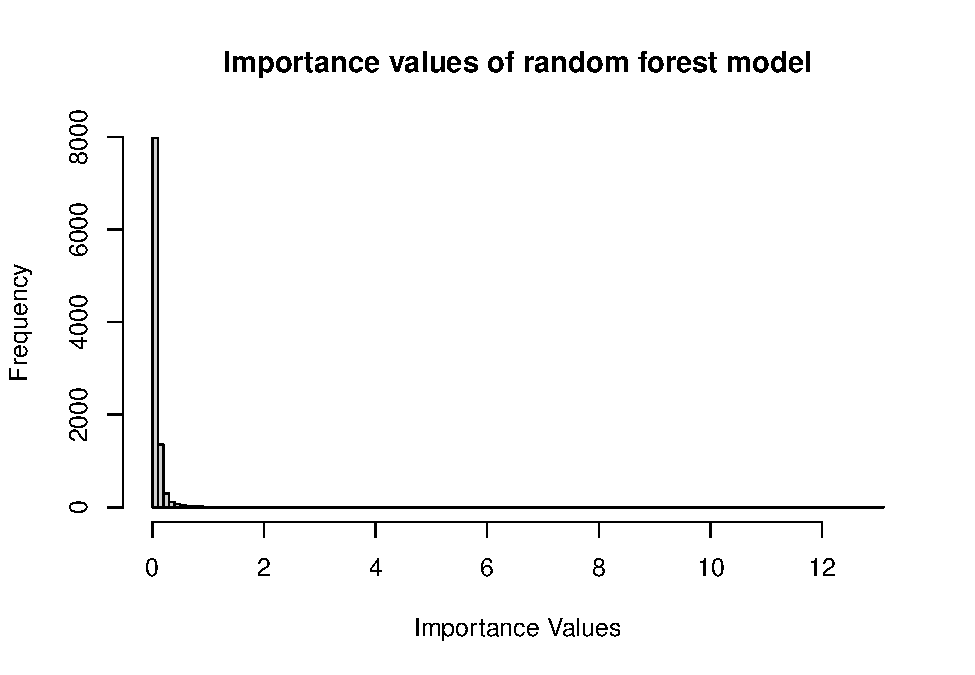
\includegraphics{STAT847_A2_Cbverghe_files/figure-latex/unnamed-chunk-3-1.pdf}
The largest number of variables (close to 8000 out of 10000) have no
importance in helping predict Perimenter Growth in the random Forest and
almost all the variable are exhausted before reaching an importance
value of 1. However there are a few genes that have an extremely high
importance value resulting in the histogram's maximum range reaching up
to 12.

Therefore, there are very few genes that have a relatively high
importance value in the determination of Perimeter Growth in the random
Forest over the 10000 genes provided. \newpage

\begin{enumerate}
\def\labelenumi{\arabic{enumi}.}
\setcounter{enumi}{2}
\tightlist
\item
  (0 marks) Use the following code to make a new dataset that only
  includes perimeter growth and the most important 50 genetic variables
  from random forest for perimeter growth. \texttt{mod2} is the name of
  the \texttt{randomForest()} output in this case.
\end{enumerate}

\begin{Shaded}
\begin{Highlighting}[]
\CommentTok{\# Set a cutoff of the 50th most important variable}
\NormalTok{cutoff }\OtherTok{=} \FunctionTok{rev}\NormalTok{(}\FunctionTok{sort}\NormalTok{(forest}\SpecialCharTok{$}\NormalTok{importance))[}\DecValTok{50}\NormalTok{]}

\CommentTok{\# Keep only those 50 variables}
\NormalTok{idx }\OtherTok{=} \FunctionTok{which}\NormalTok{(forest}\SpecialCharTok{$}\NormalTok{importance }\SpecialCharTok{\textgreater{}=}\NormalTok{ cutoff)}
\NormalTok{genes\_imp }\OtherTok{=}\NormalTok{ genes[,idx]}

\NormalTok{dat\_imp }\OtherTok{=} \FunctionTok{cbind}\NormalTok{(pheno}\SpecialCharTok{$}\NormalTok{Perimeter\_Growth, genes\_imp)}
\FunctionTok{names}\NormalTok{(dat\_imp)[}\DecValTok{1}\NormalTok{] }\OtherTok{=} \StringTok{"Perimeter\_Growth"}
\end{Highlighting}
\end{Shaded}

\newpage

\begin{enumerate}
\def\labelenumi{\arabic{enumi}.}
\setcounter{enumi}{3}
\tightlist
\item
  (4 points) Using \texttt{rpart}, and this new dataset
  \texttt{dat\_imp} (or \texttt{genes\_imp}) of the 50 most important
  variables for perimeter growth, create a single regression tree of
  perimeter growth. Plot the tree with \texttt{prp} in the
  \texttt{rpart.plot} package.
\end{enumerate}

\begin{Shaded}
\begin{Highlighting}[]
\NormalTok{fit }\OtherTok{=} \FunctionTok{rpart}\NormalTok{(dat\_imp}\SpecialCharTok{$}\NormalTok{Perimeter\_Growth }\SpecialCharTok{\textasciitilde{}}\NormalTok{ ., }\AttributeTok{data =}\NormalTok{ dat\_imp)}
\FunctionTok{prp}\NormalTok{(fit)}
\end{Highlighting}
\end{Shaded}

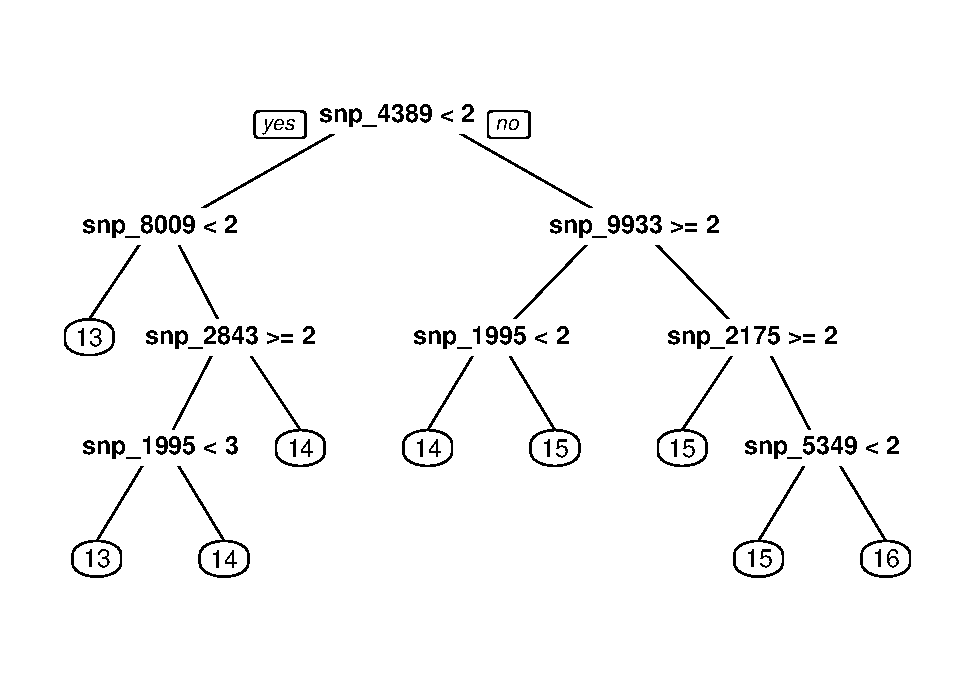
\includegraphics{STAT847_A2_Cbverghe_files/figure-latex/unnamed-chunk-5-1.pdf}
\newpage

\begin{enumerate}
\def\labelenumi{\arabic{enumi}.}
\setcounter{enumi}{4}
\tightlist
\item
  (4 marks) Using \texttt{regsubsets} in the \texttt{leaps} package, and
  the new dataset \texttt{dat\_imp} (or \texttt{genes\_imp}), use best
  subsets regression with the Adjusted R-squared criterion. Report the
  variables of the best model, their coefficients, and the adjusted
  r-squared of the model.
\end{enumerate}

\begin{Shaded}
\begin{Highlighting}[]
\NormalTok{regsub }\OtherTok{\textless{}{-}} \FunctionTok{regsubsets}\NormalTok{(dat\_imp}\SpecialCharTok{$}\NormalTok{Perimeter\_Growth }\SpecialCharTok{\textasciitilde{}}\NormalTok{ ., }\AttributeTok{data =}\NormalTok{ dat\_imp, }\AttributeTok{really.big =} \ConstantTok{TRUE}\NormalTok{, }\AttributeTok{nvmax =} \DecValTok{50}\NormalTok{, }\AttributeTok{nbest =} \DecValTok{1}\NormalTok{)}
\end{Highlighting}
\end{Shaded}

\begin{verbatim}
## Reordering variables and trying again:
\end{verbatim}

\begin{Shaded}
\begin{Highlighting}[]
\NormalTok{best\_model }\OtherTok{\textless{}{-}} \FunctionTok{which.max}\NormalTok{(}\FunctionTok{summary}\NormalTok{(regsub)}\SpecialCharTok{$}\NormalTok{adjr2)}

\NormalTok{coefficients }\OtherTok{\textless{}{-}} \FunctionTok{coef}\NormalTok{(regsub,best\_model)}
\NormalTok{coefficients }\OtherTok{\textless{}{-}}\NormalTok{ coefficients[coefficients }\SpecialCharTok{!=} \DecValTok{0}\NormalTok{]}
\NormalTok{variables }\OtherTok{\textless{}{-}} \FunctionTok{names}\NormalTok{(coefficients)[ }\SpecialCharTok{{-}}\DecValTok{1}\NormalTok{, drop }\OtherTok{=} \ConstantTok{FALSE}\NormalTok{] }
\NormalTok{best\_r2 }\OtherTok{\textless{}{-}} \FunctionTok{max}\NormalTok{(}\FunctionTok{summary}\NormalTok{(regsub)}\SpecialCharTok{$}\NormalTok{adjr2)}
\FunctionTok{print}\NormalTok{(}\StringTok{"Coefficients of the best subset model: "}\NormalTok{)}
\end{Highlighting}
\end{Shaded}

\begin{verbatim}
## [1] "Coefficients of the best subset model: "
\end{verbatim}

\begin{Shaded}
\begin{Highlighting}[]
\NormalTok{coefficients}
\end{Highlighting}
\end{Shaded}

\begin{verbatim}
## (Intercept)     snp_918    snp_2180    snp_2863    snp_4587    snp_5053 
## 12.05710692  0.29846867 -0.18916880  0.72515276 -0.16154194  0.21366132 
##    snp_5349    snp_6144    snp_6103 
##  0.17055875 -0.02866498  0.09115097
\end{verbatim}

\begin{Shaded}
\begin{Highlighting}[]
\FunctionTok{cat}\NormalTok{(}\StringTok{"}\SpecialCharTok{\textbackslash{}n}\StringTok{Variables of best subset:"}\NormalTok{,variables)}
\end{Highlighting}
\end{Shaded}

\begin{verbatim}
## 
## Variables of best subset: snp_918 snp_2180 snp_2863 snp_4587 snp_5053 snp_5349 snp_6144 snp_6103
\end{verbatim}

\begin{Shaded}
\begin{Highlighting}[]
\FunctionTok{cat}\NormalTok{(}\StringTok{"}\SpecialCharTok{\textbackslash{}n}\StringTok{ The adjusted r{-}squared value of the best subset model: "}\NormalTok{,best\_r2)}
\end{Highlighting}
\end{Shaded}

\begin{verbatim}
## 
##  The adjusted r-squared value of the best subset model:  0.4810209
\end{verbatim}

\newpage

\begin{enumerate}
\def\labelenumi{\arabic{enumi}.}
\setcounter{enumi}{5}
\tightlist
\item
  (4 marks) Run a PCA on the 50 important variables in
  \texttt{genes\_imp}. Report the total (cumulative) variance explained
  by the first 10 principal components. Plot a scree plot.
\end{enumerate}

\begin{Shaded}
\begin{Highlighting}[]
\NormalTok{PCA }\OtherTok{\textless{}{-}} \FunctionTok{princomp}\NormalTok{(genes\_imp)}

\FunctionTok{print}\NormalTok{(}\FunctionTok{cumsum}\NormalTok{(PCA}\SpecialCharTok{$}\NormalTok{sdev}\SpecialCharTok{\^{}}\DecValTok{2} \SpecialCharTok{/} \FunctionTok{sum}\NormalTok{(PCA}\SpecialCharTok{$}\NormalTok{sdev}\SpecialCharTok{\^{}}\DecValTok{2}\NormalTok{))[}\DecValTok{1}\SpecialCharTok{:}\DecValTok{10}\NormalTok{])}
\end{Highlighting}
\end{Shaded}

\begin{verbatim}
##    Comp.1    Comp.2    Comp.3    Comp.4    Comp.5    Comp.6    Comp.7    Comp.8 
## 0.3778373 0.5351362 0.6319018 0.6878164 0.7279634 0.7625764 0.7951693 0.8238089 
##    Comp.9   Comp.10 
## 0.8501684 0.8743929
\end{verbatim}

\begin{Shaded}
\begin{Highlighting}[]
\FunctionTok{fviz\_screeplot}\NormalTok{(PCA, }\AttributeTok{addlabels =} \ConstantTok{TRUE}\NormalTok{)}
\end{Highlighting}
\end{Shaded}

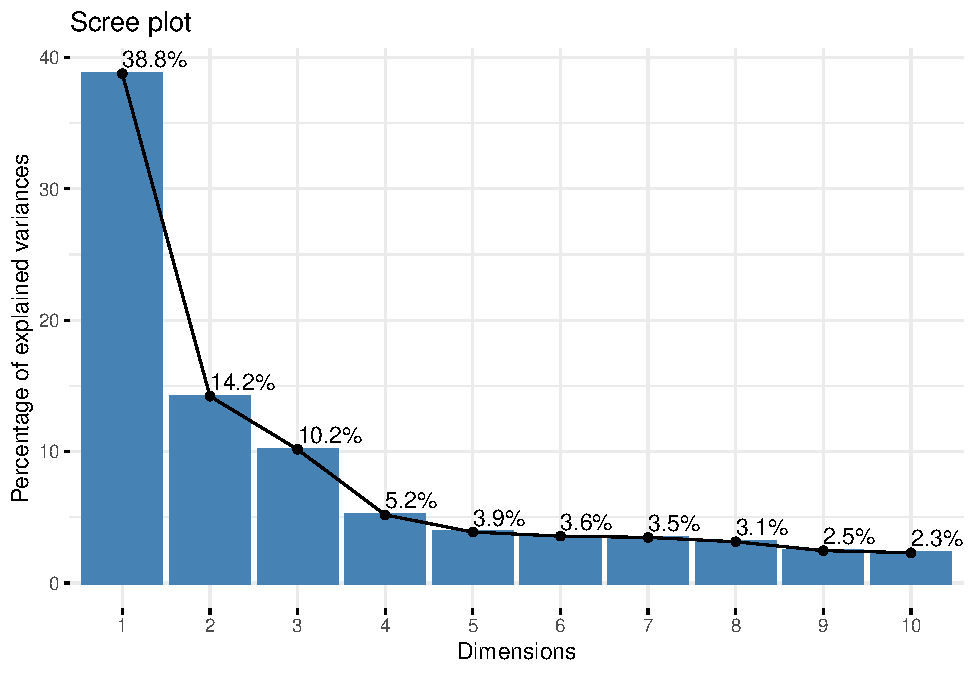
\includegraphics{STAT847_A2_Cbverghe_files/figure-latex/unnamed-chunk-8-1.pdf}
\newpage

\begin{enumerate}
\def\labelenumi{\arabic{enumi}.}
\setcounter{enumi}{6}
\tightlist
\item
  (4 marks) Build a linear model of the response variable
  \texttt{Perimeter\_Growth} using the first ten PCA dimensions from the
  previous question, and nothing else. Report the
  \texttt{summary(lm())}. Comment on the difference between this model's
  adjusted R-squared and how the adjusted r-squared values for the top
  10 PCs and the best subsets model are about the same.
\end{enumerate}

\begin{Shaded}
\begin{Highlighting}[]
\NormalTok{comp\_df }\OtherTok{=} \FunctionTok{data.frame}\NormalTok{(}\AttributeTok{Perimeter\_Growth =}\NormalTok{ dat\_imp}\SpecialCharTok{$}\NormalTok{Perimeter\_Growth, PCA}\SpecialCharTok{$}\NormalTok{scores[,}\DecValTok{1}\SpecialCharTok{:}\DecValTok{10}\NormalTok{])}
\NormalTok{pca\_lm }\OtherTok{=} \FunctionTok{lm}\NormalTok{(dat\_imp}\SpecialCharTok{$}\NormalTok{Perimeter\_Growth }\SpecialCharTok{\textasciitilde{}}\NormalTok{., }\AttributeTok{data =}\NormalTok{ comp\_df)}
\FunctionTok{summary}\NormalTok{(pca\_lm)}
\end{Highlighting}
\end{Shaded}

\begin{verbatim}
## 
## Call:
## lm(formula = dat_imp$Perimeter_Growth ~ ., data = comp_df)
## 
## Residuals:
##     Min      1Q  Median      3Q     Max 
## -4.9381 -0.7364  0.0434  0.6699  4.3059 
## 
## Coefficients:
##              Estimate Std. Error t value Pr(>|t|)    
## (Intercept) 14.314808   0.060598 236.225  < 2e-16 ***
## Comp.1       0.241417   0.015971  15.116  < 2e-16 ***
## Comp.2       0.179648   0.024752   7.258 2.43e-12 ***
## Comp.3       0.167547   0.031558   5.309 1.93e-07 ***
## Comp.4       0.051339   0.041516   1.237  0.21703    
## Comp.5       0.022910   0.048995   0.468  0.64035    
## Comp.6      -0.010019   0.052766  -0.190  0.84951    
## Comp.7      -0.158170   0.054377  -2.909  0.00385 ** 
## Comp.8      -0.008527   0.058008  -0.147  0.88321    
## Comp.9       0.137445   0.060465   2.273  0.02361 *  
## Comp.10     -0.091184   0.063073  -1.446  0.14914    
## ---
## Signif. codes:  0 '***' 0.001 '**' 0.01 '*' 0.05 '.' 0.1 ' ' 1
## 
## Residual standard error: 1.169 on 361 degrees of freedom
## Multiple R-squared:  0.4752, Adjusted R-squared:  0.4607 
## F-statistic: 32.69 on 10 and 361 DF,  p-value: < 2.2e-16
\end{verbatim}

\begin{Shaded}
\begin{Highlighting}[]
\FunctionTok{cat}\NormalTok{(}\StringTok{"Adjusted R{-}squared of linear model using 10 PCA dimension:"}\NormalTok{, }\FunctionTok{summary}\NormalTok{(pca\_lm)}\SpecialCharTok{$}\NormalTok{adj.r.squared)}
\end{Highlighting}
\end{Shaded}

\begin{verbatim}
## Adjusted R-squared of linear model using 10 PCA dimension: 0.4606695
\end{verbatim}

\begin{Shaded}
\begin{Highlighting}[]
\FunctionTok{cat}\NormalTok{(}\StringTok{"}\SpecialCharTok{\textbackslash{}n}\StringTok{Adjusted R{-}squared of best subsets regression model:"}\NormalTok{, best\_r2)}
\end{Highlighting}
\end{Shaded}

\begin{verbatim}
## 
## Adjusted R-squared of best subsets regression model: 0.4810209
\end{verbatim}

Best subset regression aims to maximize the adjusted R-squared value,
which represents the proportion of variance in the dependent variable
explained by the predictors. Similarly, PCA selects principal components
that capture the maximum variance in the data. Thus, both methods strive
to optimize the explained variance, resulting in similar adjusted
R-squared value.

\newpage

\begin{enumerate}
\def\labelenumi{\arabic{enumi}.}
\setcounter{enumi}{7}
\tightlist
\item
  (4 marks) Describe briefly one advantage and one disadvantage of the
  PCA-based model over the best subsets model. (There are several
  correct answers, but only the first two will be marked).
\end{enumerate}

One advantage PCA-based models have over best subsets models ivolve its
computational efficiency. Best subset regression involves searching
through all possible subsets of predictors, which can be computationally
expensive and time consuming, especially for large datasets with many
predictors. PCA, on the other hand, involves eigenvalue or singular
value decomposition, which is computationally efficient.

One disadvantage on the other hand involves its information loss. PCA
aims to capture maximum variance in the data, but this does not mean
that it is most relevant information for predicting the target variable.
Important predictive information may be lost during the dimensionality
reduction, resulting in suboptimal model performance.

\newpage

\begin{enumerate}
\def\labelenumi{\arabic{enumi}.}
\setcounter{enumi}{8}
\tightlist
\item
  (4 marks) The variance inflation factor of an explanatory variable in
  a model is a function of how collinear that variable is with the over
  explanatory variables in the model are. The higher the number, the
  more collinear and the most the variance estimates of the slopes are
  being inflated by including that variable. We can find the variable
  inflation factor with \texttt{vif(lm())}, where \texttt{vif} is found
  in the \texttt{car} package.
\end{enumerate}

Find the \texttt{vif()} of both the PCA-based model and best-subsets
model.

Report the VIFs for both models and briefly explain why the PCA-based
model has such low inflation factors (1 is the lowest possible).

\begin{Shaded}
\begin{Highlighting}[]
\FunctionTok{vif}\NormalTok{(pca\_lm)}
\end{Highlighting}
\end{Shaded}

\begin{verbatim}
##  Comp.1  Comp.2  Comp.3  Comp.4  Comp.5  Comp.6  Comp.7  Comp.8  Comp.9 Comp.10 
##       1       1       1       1       1       1       1       1       1       1
\end{verbatim}

\begin{Shaded}
\begin{Highlighting}[]
\NormalTok{data\_subset }\OtherTok{\textless{}{-}}\NormalTok{ dat\_imp[, }\FunctionTok{c}\NormalTok{(}\StringTok{"Perimeter\_Growth"}\NormalTok{, variables)]}
\FunctionTok{vif}\NormalTok{(}\FunctionTok{lm}\NormalTok{(dat\_imp}\SpecialCharTok{$}\NormalTok{Perimeter\_Growth }\SpecialCharTok{\textasciitilde{}}\NormalTok{., }\AttributeTok{data =}\NormalTok{ data\_subset))}
\end{Highlighting}
\end{Shaded}

\begin{verbatim}
##  snp_918 snp_2180 snp_2863 snp_4587 snp_5053 snp_5349 snp_6144 snp_6103 
## 1.138870 1.333843 1.472024 2.048521 2.523176 1.580688 1.826940 2.610587
\end{verbatim}

The PCA-based model has lower inflation factors due to PCs being
orthogonal in nature due to it aiming to capture the maximum explained
variance. As such, it reduces multicollinearity among the predictors,
leading to the lowest Variance Inflation Factors (VIFs). .

On the other hand, a linear model created from the variables from the
best subset has higher collinearity due making use of highly correlated
predicted giving rise to its higher variance inflation factor scores.

\end{document}
